\documentclass[11pt]{article}

\usepackage[margin=1in]{geometry}
\usepackage{amsmath,amssymb,amsthm,mathtools}
\usepackage{microtype}
\usepackage{enumitem}\usepackage{tikz}
\usepackage{xurl}\usepackage[hidelinks]{hyperref}
\usepackage[nameinlink,noabbrev,capitalise]{cleveref}
\AtBeginDocument{\AddToHook{env/proposition/begin}{\crefalias{theorem}{proposition}}\AddToHook{env/lemma/begin}{\crefalias{theorem}{lemma}}\AddToHook{env/corollary/begin}{\crefalias{theorem}{corollary}}\AddToHook{env/definition/begin}{\crefalias{theorem}{definition}}\AddToHook{env/remark/begin}{\crefalias{theorem}{remark}}}
\newtheorem{theorem}{Theorem}[section]
\newtheorem{proposition}[theorem]{Proposition}
\newtheorem{lemma}[theorem]{Lemma}
\newtheorem{corollary}[theorem]{Corollary}
\theoremstyle{definition}
\newtheorem{definition}[theorem]{Definition}
\theoremstyle{remark}
\newtheorem{remark}[theorem]{Remark}

\newcommand{\PP}{\mathbb P}
\newcommand{\EE}{\mathbb E}
\newcommand{\ZZ}{\mathbb Z}
\newcommand{\HH}{\mathbb H}
\newcommand{\Z}{\mathbb{Z}}
\newcommand{\cF}{\mathcal F}
\newcommand{\cH}{\mathcal H}
\newcommand{\1}{\mathbf 1}
\newcommand{\Cov}{\operatorname{Cov}}
\newcommand{\diag}{\operatorname{diag}}
\newcommand{\dist}{\operatorname{dist}}
\newcommand{\RS}{\operatorname{RS}}
\newcommand{\e}{\mathrm e}

\title{Exponential Decay for the Two-Dimensional Arboreal Gas}
\author{}
\date{}

\begin{document}
\maketitle

\begin{abstract}
We give a detailed argument for exponential decay of two-point connectivity in the
arboreal gas on finite nearest-neighbour subgraphs of $\ZZ^2$ and on the two-dimensional
torus, for every finite edge fugacity.  The argument does not use the conjectural full
negative-correlation property of the arboreal gas.  Instead, it derives two weaker
comparison principles from real stability of a vertex-field forest polynomial:
negative correlation for two edges incident to a common vertex, and monotonicity of
two-point connectivity under wiring a vertex separator.  The analytic input is the
$\HH^{0|2}$/$\HH^{2|4}$ representation of Bauerschmidt--Crawford--Helmuth--Swan
\cite{BCHS}, together with their logarithmic deformation estimate which is based on
Sabot's Mermin--Wagner theorem \cite{Sabot}.  We state every
input from \cite{BCHS} with its exact theorem/equation number and prove the additional combinatorial,
stability, conductance, and Simon--Lieb steps in full.
\end{abstract}

\paragraph{Status of the argument.}
The inputs from \cite{BCHS} quoted below are established results.  The stability argument,
separator lemma, separator-wiring comparison, effective-conductance identity, and
Simon--Lieb argument are proved in this note.  In particular, the separator-wiring
lemma is not being attributed to \cite{BCHS}.  Since this route appears to be different from
the published argument of \cite{BCHS}, it should be independently checked before being cited as
a literature theorem.

\section{Statement and notation}

Let $G=(V,E)$ be a finite graph with nonnegative edge weights $w=(w_e)_{e\in E}$.
The arboreal gas is the probability measure on spanning forests
$F\subseteq E$ defined by
\begin{equation}\label{eq:forest-measure}
 \mu_{G,w}(F)=\frac{w(F)}{Z_G(w)},\qquad
 w(F)=\prod_{e\in F}w_e,\qquad
 Z_G(w)=\sum_{F\in\cF(G)}w(F).
\end{equation}
For $x,y\in V$ write
\begin{equation}
 \tau_G(x,y)=\mu_{G,w}(x\leftrightarrow y).
\end{equation}
Zero-weight edges are deleted.  Parallel edges may be retained as distinct labelled
edges; whenever only connectivity is relevant they may equivalently be replaced by a
single edge whose weight is the sum of their weights.  Loops are always discarded.

\begin{theorem}\label{thm:main}
Fix $\beta<\infty$.  There exists $c_\beta>0$ such that, for every finite
nearest-neighbour subgraph $G\subseteq\ZZ^2$ whose edge weights satisfy
$0\le w_e\le\beta$,
\begin{equation}\label{eq:main-finite}
 \tau_G(x,y)\le 2\exp\{-c_\beta\|x-y\|_\infty\}.
\end{equation}
The same estimate holds on $\Lambda_L=(\ZZ/L\ZZ)^2$, uniformly in $L$, with
$\|x-y\|_\infty$ interpreted as toroidal $\ell^\infty$ distance.  Consequently, when
$L\gg |x|$,
\begin{equation}
 \PP_{\Lambda_L,\beta}(0\leftrightarrow x)\le C_\beta\e^{-c'_\beta |x|_2}.
\end{equation}
\end{theorem}

The proof is organized as follows.  Sections~\ref{sec:stability}--\ref{sec:separator}
prove the comparison principles.  Sections~\ref{sec:BCHS}--\ref{sec:annulus} isolate
and use the sigma-model input from \cite{BCHS}.  Section~\ref{sec:superpoly} obtains a uniform
superpolynomial two-point bound.  Sections~\ref{sec:SL}--\ref{sec:exp} upgrade this to
exponential decay.

\section{A real-stable vertex-field polynomial}\label{sec:stability}

For vertex variables $h=(h_i)_{i\in V}$ define
\begin{equation}\label{eq:PG-def}
 P_G(h)=\sum_{F\in\cF(G)}w(F)
 \prod_{T\in\operatorname{comp}(F)}\left(1+\sum_{i\in T}h_i\right).
\end{equation}
This is exactly the forest polynomial in
\cite[Theorem~2.1, (2.8)]{BCHS}.  Notice directly from \eqref{eq:PG-def} that
$P_G$ is multi-affine.  Moreover every coefficient is strictly positive: the empty
forest contributes $1$ to the coefficient of every square-free monomial
$\prod_{i\in A}h_i$.

\subsection{Real stability and a differential-operator formula}

\begin{definition}
A polynomial $p\in\mathbb R[z_1,\dots,z_n]$ is \emph{real stable} if
$p(z_1,\dots,z_n)\neq0$ whenever $\operatorname{Im}z_j>0$ for all $j$.
\end{definition}

Let $L_w$ denote the positive weighted graph Laplacian,
\begin{equation}
 (L_w)_{ii}=\sum_{j:ij\in E}w_{ij},\qquad
 (L_w)_{ij}=-w_{ij}\quad(i\neq j).
\end{equation}
Set
\begin{equation}\label{eq:det-poly}
 D_G(h)=\det\bigl(L_w+\diag(1+h_i:i\in V)\bigr).
\end{equation}

\begin{lemma}[Differential-operator identity]\label{lem:operator-identity}
One has
\begin{equation}\label{eq:operator-identity}
 P_G(h)=
 \prod_{\{i,j\}\in E}
 \left(1-w_{ij}\partial_{h_i}\partial_{h_j}\right)D_G(h).
\end{equation}
\end{lemma}

\begin{proof}
We give the Grassmann calculation explicitly, both to fix signs and to make clear the
relation with \cite{BCHS}.  Use Grassmann generators $(\xi_i,\eta_i)_{i\in V}$ and put
$q_i=\xi_i\eta_i$.  The authors of \cite{BCHS} define
\begin{equation}
 z_i=1-q_i
\end{equation}
in their equation~(2.2), and their equation~(2.3) reads
\begin{equation}
 1+u_i\cdot u_j
 =-\xi_i\eta_j-\xi_j\eta_i+q_i+q_j-q_iq_j.
\end{equation}
Their hyperbolic Grassmann integral includes the factor
$z_i^{-1}=1+q_i=\exp(q_i)$ at each vertex; see \cite[(2.5)]{BCHS}.  Their action and
expectation are (2.6)--(2.7) \cite[(2.2)--(2.7)]{BCHS}.

For an undirected edge $ij$, the edge part of $\exp(-H_{w,h})$ is therefore
\begin{equation}
 \exp\!\left(w_{ij}(1+u_i\cdot u_j)\right)
 =\exp\!\left[w_{ij}
   (-\xi_i\eta_j-\xi_j\eta_i+q_i+q_j-q_iq_j)\right].
\end{equation}
Since $q_iq_j$ is nilpotent and even, this splits as a quadratic exponential times
$1-w_{ij}q_iq_j$.  The vertex term $h_i(z_i-1)=-h_iq_i$ contributes
$\exp(h_iq_i)$ to $\exp(-H_{w,h})$, while the measure factor contributes
$\exp(q_i)$.  Collecting all quadratic terms gives exactly
\begin{equation}
 \sum_{i,j}\xi_i
 \bigl(L_w+\diag(1+h)\bigr)_{ij}\eta_j.
\end{equation}
Consequently the unnormalised partition function can be written as
\begin{equation}\label{eq:grassmann-operator}
 [1]_{w,h}
 =\int d(\xi,\eta)\,
 \exp\{\xi^T(L_w+\diag(1+h))\eta\}
 \prod_{ij\in E}(1-w_{ij}q_iq_j),
\end{equation}
where $d(\xi,\eta)$ denotes the ordinary Berezin coefficient extraction.
The fermionic Gaussian identity
\begin{equation}
 \int d(\xi,\eta)\,\exp(\xi^TA\eta)=\det A
\end{equation}
is \cite[Lemma~2.11, (2.74)]{BCHS}.
Furthermore, differentiating the Gaussian determinant with respect to $h_i$ inserts
$q_i$ under the integral.  Thus insertion of $q_iq_j$ is
$\partial_{h_i}\partial_{h_j}D_G(h)$.  Expanding the product in
\eqref{eq:grassmann-operator} therefore gives the right-hand side of
\eqref{eq:operator-identity}.

Finally, \cite[Theorem~2.1]{BCHS} identifies $[1]_{w,h}$ with the forest sum
\eqref{eq:PG-def}.  This proves \eqref{eq:operator-identity}.
\end{proof}

\begin{lemma}\label{lem:PG-stable}
The polynomial $P_G$ is real stable.
\end{lemma}

\begin{proof}
First, $D_G$ is real stable.  Indeed, if $\operatorname{Im}h_i>0$ for every $i$ and
$M=L_w+\diag(1+h)$, then for every nonzero $v\in\mathbb C^V$,
\begin{equation}
 \operatorname{Im}(v^*Mv)=\sum_i(\operatorname{Im}h_i)|v_i|^2>0.
\end{equation}
Hence $Mv\neq0$, so $\det M\neq0$.

We next show that, on the space of multi-affine polynomials, each operator
\begin{equation}
 T_{ij}=1-c\,\partial_{h_i}\partial_{h_j},\qquad c\ge0,
\end{equation}
preserves stability.  We use the finite-dimensional
characterisation \cite[Theorem~1.1]{BB}.  For the degree box
$\kappa=(1,\dots,1)$, the algebraic symbol of $T_{ij}$ is
\begin{equation}\begin{aligned}
 G_{T_{ij}}(z,w)
 &=T_{ij}\prod_{k}(z_k+w_k)\\
 &=\prod_{k\neq i,j}(z_k+w_k)
   \bigl((z_i+w_i)(z_j+w_j)-c\bigr).
\end{aligned}\end{equation}
If all $z_k,w_k$ lie in the open upper half-plane, then every $z_k+w_k$ does also.
The product of two numbers in the open upper half-plane cannot be a nonnegative real
number: the sum of their arguments lies strictly between $0$ and $2\pi$ and cannot be
$0$ or $2\pi$.  Thus the displayed symbol is stable.  By
\cite[Theorem~1.1]{BB}, $T_{ij}$ preserves stability (or sends a stable polynomial to
zero).  It cannot annihilate the polynomial in our application because the top
monomial $\prod_i h_i$ survives.

Apply this to every factor in \eqref{eq:operator-identity}.  Since $D_G$ is stable,
so is $P_G$.
\end{proof}

We will repeatedly use elementary closure properties of stability: differentiation,
real specialization, real translation, and identification of variables preserve
stability, allowing the zero polynomial.  Identification and translation follow
immediately from the definition.  Real specialization is obtained as a limit from
specialization at $a+i\varepsilon$ and Hurwitz's theorem; differentiation follows by
applying the univariate Gauss--Lucas theorem on each line in a positive imaginary
direction, followed again by Hurwitz.  These are also standard consequences of the
stability theory developed in \cite{BB,BBL}.

For multi-affine polynomials we need the following exact criterion.

\begin{lemma}[Rayleigh criterion]\label{lem:rayleigh}
If $p\in\mathbb R[z_1,\dots,z_n]$ is multi-affine and real stable, then for all real
$x$ and all $i,j$,
\begin{equation}\label{eq:rayleigh}
 \Delta_{ij}p(x):=(\partial_i p)(x)(\partial_j p)(x)
 -p(x)(\partial_i\partial_jp)(x)\ge0.
\end{equation}
\end{lemma}

\begin{proof}
This is
\cite[Theorem~4.1]{BBL}.  In the bivariate restriction
$p=a z_i z_j+b z_i+c z_j+d$, the Rayleigh difference is the constant $bc-ad$.
\end{proof}

\subsection{Incident-edge negative correlation}

\begin{proposition}[Incident-edge negative correlation]\label{prop:incident-NC}
Let $e=\rho i$ and $f=\rho j$ be two distinct edges incident to a common vertex
$\rho$.  Then
\begin{equation}\label{eq:incident-NC}
 \mu_G(e,f\in F)\le \mu_G(e\in F)\mu_G(f\in F).
\end{equation}
The same statement holds after conditioning on the inclusion of any prescribed
forest edge set.
\end{proposition}

\begin{proof}
Delete $\rho$ and call the resulting graph $H$.  Keep all original edges of $H$.
For each $v\in V(H)$, let $h_v$ be the total weight of edges from $\rho$ to $v$;
if parallel edges are to be distinguished, one may first keep separate variables and
then specialize them.

Fix a forest $F_H$ of $H$.  For each tree $T$ of $F_H$, a forest on $G$ may use at
most one edge from $\rho$ into $T$, and the total weight of the choices is
$1+\sum_{v\in T}h_v$.  Hence the partition function of $G$ is exactly $P_H(h)$.
For two specific incident edges, differentiation with respect to their individual
weights gives
\begin{equation}
 \mu_G(e\in F)=\frac{w_e\partial_e Z_G}{Z_G},\qquad
 \mu_G(e,f\in F)=\frac{w_ew_f\partial_e\partial_f Z_G}{Z_G}.
\end{equation}
Thus \eqref{eq:incident-NC} is precisely the Rayleigh inequality
\eqref{eq:rayleigh} for the corresponding variables of the real-stable polynomial
$P_H$.

If a prescribed forest $A$ is conditioned to be present, its edges may be contracted:
for every forest $F\supset A$, $F/A$ is a forest on $G/A$, and
$w(F)=w(A)w(F/A)$.  Therefore the conditional law is the arboreal gas on the
contracted weighted multigraph $G/A$.  Applying the first part there proves the
conditional statement.
\end{proof}

\section{A separator-wiring comparison}\label{sec:separator}

The main replacement for arbitrary edge negative correlation is a comparison that is
special to vertex separators.

\subsection{An elementary rational Pick lemma}

\begin{lemma}\label{lem:rational-pick}
Let $R\in\mathbb R(t)$ have no pole in the open upper half-plane and satisfy
$\operatorname{Im}R(z)\le0$ whenever $\operatorname{Im}z>0$.  Assume $R$ has a finite
real limit $c$ at infinity.  Then every pole of $R$ is real and simple and
\begin{equation}\label{eq:pick-expansion}
 R(t)=c+\sum_{\nu}\frac{d_\nu}{t-\lambda_\nu},
 \qquad d_\nu\ge0,\quad \lambda_\nu\in\mathbb R.
\end{equation}
Consequently, on every real interval containing no pole,
\begin{equation}
 R'(t)=-\sum_\nu\frac{d_\nu}{(t-\lambda_\nu)^2}\le0.
\end{equation}
\end{lemma}

\begin{proof}
Because $R$ has real coefficients, every nonreal pole occurs with its complex
conjugate.  A pole in the lower half-plane would therefore force one in the upper
half-plane, which is impossible.  Hence all poles are real.

Let $\lambda$ be a pole of order $m$ with real leading Laurent coefficient $a\neq0$.
For $z=\lambda+r\e^{i\theta}$ with $0<\theta<\pi$,
\begin{equation}
 R(z)=a r^{-m}\e^{-im\theta}+O(r^{-m+1}).
\end{equation}
If $m\ge2$, the imaginary part of the leading term changes sign as $\theta$ varies in
$(0,\pi)$, contradicting $\operatorname{Im}R\le0$.  Thus $m=1$.  For a simple pole,
\begin{equation}
 \operatorname{Im}\frac{a}{z-\lambda}
 =-a\frac{\operatorname{Im}z}{|z-\lambda|^2},
\end{equation}
so $a\ge0$.  Subtracting the simple pole terms leaves an entire rational function,
hence a polynomial.  The finite limit at infinity forces that polynomial to be the
constant $c$.  This proves \eqref{eq:pick-expansion} and the derivative formula.
\end{proof}

\subsection{A stable-polynomial separator lemma}

\begin{lemma}[Stable separator lemma]\label{lem:stable-separator}
Let
\begin{equation}
 p(x,y,s_1,\dots,s_m)
\end{equation}
be a real-stable multi-affine polynomial with strictly positive coefficients.  Suppose
the coefficient of $s_1\cdots s_m$ is
\begin{equation}\label{eq:top-s-coeff}
 [s_1\cdots s_m]p=c(x+A)(y+B),\qquad c,A,B>0.
\end{equation}
Then
\begin{equation}\label{eq:separator-algebraic-conclusion}
 p(-A,-B,0,\dots,0)\ge0.
\end{equation}
\end{lemma}

\begin{proof}
Identify $s_1=\cdots=s_m=t$ and translate $x,y$:
\begin{equation}\label{eq:f-UVWX}
 f(x,y,t):=p(x-A,y-B,t,\dots,t)
 =U(t)xy+V(t)x+W(t)y+X(t).
\end{equation}
The closure properties stated after \cref{lem:PG-stable} imply that $f$ is real
stable.  By \eqref{eq:top-s-coeff}, the coefficient of $t^m$ in $f$ is $cxy$.
Therefore
\begin{equation}\label{eq:degree-UVWX}
 \deg U=m,\qquad \deg V,\deg W,\deg X\le m-1.
\end{equation}

\paragraph{Step 1: $\deg X\le m-2$.}
Apply $\partial_t^{m-1}$ to $f$.  Up to positive factorial constants, the result has
the form
\begin{equation}
 g(x,y,t)=(kt+\ell)xy+vx+wy+\chi,
 \qquad k>0.
\end{equation}
It is again real stable.  By the Rayleigh criterion \eqref{eq:rayleigh},
\begin{equation}
 \Delta_{xy}g=vw-\chi(kt+\ell)\ge0
\end{equation}
for every real $t$.  Since $k>0$, this is possible only if $\chi=0$.  Hence
\begin{equation}\label{eq:X-degree}
 \deg X\le m-2.
\end{equation}
For $m=1$, this says $X\equiv0$, and the lemma follows immediately.  We henceforth
assume $m\ge2$.

\paragraph{Step 2: the sign and degree of $V$.}
Before translating $x,y$, write
\begin{equation}\label{eq:a-decomp}
 p(x,y,t,\dots,t)=a_0(t)+a_1(t)x+a_2(t)y+a_{12}(t)xy.
\end{equation}
Then
\begin{equation}
 U=a_{12},\qquad V=a_1-Ba_{12}.
\end{equation}
By \eqref{eq:top-s-coeff}, the leading coefficients of $a_{12}$ and $a_1$ are
$c$ and $cB$, respectively.

The polynomial
\begin{equation}
 \partial_xp(x,y,t,\dots,t)=a_1(t)+y a_{12}(t)
\end{equation}
is stable.  Hence, for $\operatorname{Im}t>0$, its root in $y$ cannot belong to the
upper half-plane.  Equivalently,
\begin{equation}\label{eq:r-pick}
 r(t):=\frac{a_{12}(t)}{a_1(t)}
\end{equation}
maps the upper half-plane into the closed lower half-plane.

Also $a_1$ is a univariate real-stable polynomial: differentiate $p$ in $x$ and
specialize $y=0$ and $s_1=\cdots=s_m=t$.  Since $a_1$ has strictly positive
coefficients, all of its zeros are strictly negative.  (Real stability plus real
coefficients makes all zeros real; positive coefficients exclude nonnegative zeros.)
Moreover $r(t)\to1/B$ as $t\to\infty$.  Applying
\cref{lem:rational-pick}, and writing the negative poles as $-\lambda_\nu$, gives
\begin{equation}\label{eq:r-expansion}
 r(t)=\frac1B+\sum_\nu\frac{d_\nu}{t+\lambda_\nu},
 \qquad d_\nu\ge0,\quad \lambda_\nu>0.
\end{equation}
Therefore either every $d_\nu=0$, in which case $V\equiv0$, or
\begin{equation}\label{eq:V-negative}
 V(t)=a_1(t)(1-Br(t))
 =-B a_1(t)\sum_\nu\frac{d_\nu}{t+\lambda_\nu}<0
 \qquad(t\ge0).
\end{equation}
In the latter case $\deg V=m-1$: after putting the right side over the denominator
$a_1$, the leading coefficient is a nonzero negative multiple of
$\sum_
u d_\nu$.

\paragraph{Step 3: the case $V\not\equiv0$.}
Specialize $y=0$ in \eqref{eq:f-UVWX}.  The stable polynomial
\begin{equation}
 V(t)x+X(t)
\end{equation}
has the unique root in $x$
\begin{equation}
 R(t):=-\frac{X(t)}{V(t)}.
\end{equation}
Thus $R$ maps the upper half-plane into the closed lower half-plane.  By
\eqref{eq:V-negative}, $V$ has no zero on $[0,\infty)$, so $R$ has no pole there.
By \cref{lem:rational-pick}, $R'(t)\le0$ for $t\ge0$.  By
\eqref{eq:X-degree} and $\deg V=m-1$,
\begin{equation}
 \lim_{t\to\infty}R(t)=0.
\end{equation}
Hence $R(t)\ge0$ for all $t\ge0$.  Since $V(t)<0$ there,
\begin{equation}
 X(t)=-V(t)R(t)\ge0.
\end{equation}
In particular $X(0)\ge0$.

\paragraph{Step 4: the case $V\equiv0$.}
Because the original $p$ is multi-affine in each $s_j$, after diagonal specialization
we have the exact identity
\begin{equation}\label{eq:delta-diagonal}
 \Delta_{x,t}f
 =\sum_{j=1}^m
 \left.\Delta_{x,s_j}p(x-A,y-B,s_1,\dots,s_m)
 \right|_{s_1=\cdots=s_m=t}.
\end{equation}
Indeed $\partial_t f=\sum_j\partial_{s_j}p$ and similarly for the mixed derivative.
Every term on the right is nonnegative for real arguments by
\cref{lem:rayleigh}.  If $V=0$, direct calculation from
\eqref{eq:f-UVWX} gives
\begin{equation}
 \Delta_{x,t}f
 =y^2(UW'-WU')+y(UX'-XU').
\end{equation}
A real quadratic polynomial of the form $ay^2+by$ that is nonnegative for every
real $y$ must have $b=0$.  Therefore
\begin{equation}
 UX'-XU'=0.
\end{equation}
Thus $(X/U)'=0$ wherever $U\neq0$, hence as a rational identity $X/U$ is constant.
Since $\deg X<\deg U$ by \eqref{eq:X-degree}, that constant is zero and
$X\equiv0$.

In both cases $X(0)\ge0$.  By the definition \eqref{eq:f-UVWX},
$X(0)=p(-A,-B,0,\dots,0)$, proving the lemma.
\end{proof}

\subsection{Wiring a separator increases connectivity}

\begin{proposition}[Separator-wiring monotonicity]\label{prop:separator-wiring}
Let $a,b\in V(G)$ and let $S\subseteq V(G)\setminus\{a,b\}$ be a vertex separator:
every $a$--$b$ path in $G$ meets $S$.  Let $G/S$ be the weighted multigraph obtained
by identifying all vertices of $S$ to a single vertex $\rho$.  Then
\begin{equation}\label{eq:separator-wiring}
 \tau_G(a,b)\le \tau_{G/S}(a,b).
\end{equation}
\end{proposition}

\begin{proof}
Let $\Gamma=G/S$, and define
\begin{equation}
 r_a=\PP_\Gamma(a\nleftrightarrow\rho),\qquad
 r_b=\PP_\Gamma(b\nleftrightarrow\rho).
\end{equation}
Both are positive because the empty forest has positive weight.

In the polynomial $P_G$, set all vertex variables outside $\{a,b\}\cup S$ to zero,
and denote the resulting polynomial by
\begin{equation}
 p(x,y,(s_v)_{v\in S}).
\end{equation}
By \cref{lem:PG-stable}, it is real stable; its coefficients are strictly positive.
At $s=0$, a forest in which $a,b$ are disconnected contributes
$(1+x)(1+y)$ from their two components, while a forest in which they are connected
contributes $1+x+y$.  Therefore
\begin{equation}\label{eq:p-szero}
 p(x,y,0)=Z_G\bigl(1+x+y+(1-\tau_G(a,b))xy\bigr).
\end{equation}

Now take the coefficient of $\prod_{v\in S}s_v$.  In the product over forest
components in \eqref{eq:PG-def}, this monomial occurs exactly when distinct vertices
of $S$ lie in distinct forest components; its coefficient in that case is $1$.
Identifying those components at one point gives a weight-preserving bijection with
forests of $\Gamma$ (keeping parallel edges labelled).  Conversely, splitting $\rho$
back into the vertices of $S$ takes every forest of $\Gamma$ to a forest in which the
vertices of $S$ are in distinct components: if two of the resulting branches were
connected away from $\rho$, the original forest on $\Gamma$ would contain a cycle.

After extracting the $S$-monomial, an $x$ factor is available exactly when the tree
containing $a$ contains no vertex of $S$, i.e. exactly when $a\nleftrightarrow\rho$
in $\Gamma$; similarly for $b$.  Since $S$ separates $a,b$, the vertices $a,b$ lie in
different connected components of $G\setminus S$.  Thus $\Gamma$ is a one-vertex
union at $\rho$ of edge-disjoint subgraphs containing $a$ and $b$.  The forest
partition function factors over a one-vertex union: a set of edges is a forest in the
union iff its restriction to every piece is a forest, and the weights multiply.
Hence the events $a\nleftrightarrow\rho$ and $b\nleftrightarrow\rho$ are independent
under the corresponding product decomposition.  It follows that
\begin{equation}\label{eq:p-topS}
 [\prod_{v\in S}s_v]p
 =Z_\Gamma(1+r_ax)(1+r_by).
\end{equation}

Apply \cref{lem:stable-separator} with $A=r_a^{-1}$ and $B=r_b^{-1}$.  From
\eqref{eq:p-szero},
\begin{equation}\begin{aligned}
 0&\le p(-r_a^{-1},-r_b^{-1},0)\\
 &=Z_G(r_ar_b)^{-1}
 \left[(1-r_a)(1-r_b)-\tau_G(a,b)\right].
\end{aligned}\end{equation}
Therefore
\begin{equation}\label{eq:tau-less-product}
 \tau_G(a,b)\le(1-r_a)(1-r_b).
\end{equation}
Finally, by the same one-vertex factorization at $\rho$,
\begin{equation}
 \tau_\Gamma(a,b)
 =\PP_\Gamma(a\leftrightarrow\rho)\PP_\Gamma(b\leftrightarrow\rho)
 =(1-r_a)(1-r_b).
\end{equation}
Combining with \eqref{eq:tau-less-product} proves \eqref{eq:separator-wiring}.
\end{proof}

\section{Precisely stated inputs from \texorpdfstring{\cite{BCHS}}{BCHS}}\label{sec:BCHS}

This section records the sigma-model facts used later.  We keep the notation of \cite{BCHS} as
much as possible and indicate exactly how each statement enters.

\subsection{Forest and pinned horospherical representations}

\cite[Theorem~2.1, (2.8)]{BCHS} states that the $\HH^{0|2}$ partition function is exactly
\eqref{eq:PG-def}.  Their Corollary~2.2 gives,
for nonnegative edge weights,
\begin{equation}\label{eq:BCHS-ferm-connect}
 \PP_w(i\leftrightarrow j)=\langle\xi_i\eta_j\rangle_w,
\end{equation}
which is one of the equalities in
\cite[Corollary~2.2, (2.11)]{BCHS}.

For the $\HH^{2|4}$ model with nonnegative irreducible edge weights and nonnegative
vertex pinning $h$, \cite[Proposition~2.9]{BCHS} gives the horospherical $(t,s)$ integral.
Their equations (2.59)--(2.62) show in particular that, conditionally on $t$, the
$s$-field is a centered Gaussian whose quadratic form is the weighted Laplacian with
conductances $w_{ij}\e^{t_i+t_j}$ plus the pinning term; see
\cite[Proposition~2.9, (2.59)--(2.62)]{BCHS}.  \cite[Corollary~2.10]{BCHS} gives
\begin{equation}\label{eq:BCHS-moments-unpinned}
 \langle\e^{t_i}\rangle_{w,h}
 =\langle\e^{2t_i}\rangle_{w,h},
 \qquad
 \langle\e^{3t_i}\rangle_{w,h}=1,
\end{equation}
and
\begin{equation}\label{eq:BCHS-s-fermion}
 \langle s_is_j\e^{t_i+t_j}\rangle_{w,h}
 =\langle\xi_i\eta_j\rangle_{w,h};
\end{equation}
these are
\cite[Corollary~2.10, (2.63)--(2.64)]{BCHS}.

For a chosen vertex $\rho$, the pinned model is defined in \cite[(2.77)--(2.78)]{BCHS}.
Proposition~2.12, especially (2.79)--(2.80), identifies pinned and unpinned
expectations \cite[Proposition~2.12, (2.79)--(2.80)]{BCHS}.  Corollary~2.13 then
gives the pinned $t$-density, equations (2.84)--(2.85)
\cite[Corollary~2.13, (2.84)--(2.85)]{BCHS}.  Most importantly, Corollary~2.14 states
\begin{equation}\label{eq:BCHS-pinned-connect}
 \PP_w(\rho\leftrightarrow i)=\langle\e^{t_i}\rangle_w^\rho,
 \qquad
 \langle\e^{3t_i}\rangle_w^\rho=1;
\end{equation}
these are
\cite[Corollary~2.14, (2.86)--(2.87)]{BCHS}.  Combining the pinned construction with
Corollary~2.10 also gives
\begin{equation}\label{eq:BCHS-pinned-second}
 \langle\e^{2t_i}\rangle_w^\rho
 =\langle\e^{t_i}\rangle_w^\rho
 =\PP_w(\rho\leftrightarrow i).
\end{equation}
Indeed the pinned measure is the vertex-pinned instance of Proposition~2.9 on
$V\setminus\{\rho\}$, as explained in \cite{BCHS} immediately before and in
Corollary~2.13.

\subsection{A Green-function identity}

Let $U_i=\e^{t_i}$ and $U_\rho=1$.  In the pinned model, let $A(t)$ be the grounded
Laplacian on $V\setminus\{\rho\}$ with conductances
\begin{equation}\label{eq:conductances}
 c_{ij}=w_{ij}U_iU_j.
\end{equation}
Set
\begin{equation}\label{eq:H-def}
 H(t)=D_U^{-1}A(t)D_U^{-1},
 \qquad D_U=\diag(U_i:i\neq\rho).
\end{equation}
By \cite[Proposition~2.9, (2.59)]{BCHS}, conditionally on $t$ the $s$-field has
covariance $A(t)^{-1}$.  Hence
\begin{equation}\label{eq:conditional-s}
 \EE[s_is_jU_iU_j\mid t]=(H(t)^{-1})_{ij}.
\end{equation}
Averaging and using \cite[(2.64)]{BCHS} gives
\begin{equation}\label{eq:H-fermion}
 \EE_w^\rho(H^{-1})_{ij}
 =\langle\xi_i\eta_j\rangle_w^\rho.
\end{equation}

We now identify the pinned fermionic expectation combinatorially.

\begin{lemma}\label{lem:pinned-green-event}
For $i,j\neq\rho$,
\begin{equation}\label{eq:pinned-green-event}
 \EE_w^\rho(H^{-1})_{ij}
 =\PP_w(i\leftrightarrow j,\ i\nleftrightarrow\rho).
\end{equation}
\end{lemma}

\begin{proof}
Equation \eqref{eq:H-fermion} reduces the claim to the corresponding identity for the
pinned $\HH^{0|2}$ expectation.  By \cite[Proposition~2.12, (2.79)]{BCHS}, pinning
at $\rho$ inserts the factor $1-z_\rho=\xi_\rho\eta_\rho$ in the unpinned
Grassmann integral.  Thus the numerator of
$\langle\xi_i\eta_j\rangle_w^\rho$ contains the insertion
\begin{equation}
 \xi_\rho\eta_\rho\,\xi_i\eta_j.
\end{equation}
Expand the interaction by forests as in the proof of \cite[Theorem~2.1]{BCHS} (see
\cite[Section~2.3]{BCHS}; in particular Lemma~2.4 and equations (2.28)--(2.36)).  A nonzero term
with $\xi_i\eta_j$ requires $i,j$ to lie in the same tree; the insertion
$\xi_\rho\eta_\rho$ forces $\rho$ to lie in a different tree.  For every such
forest the Grassmann integral of the marked components equals $1$, by the same
leaf-removal/factorization calculation used in \cite[Lemma~2.4]{BCHS}.  Forests not satisfying
these connectivity requirements give zero because some marked component is missing a
Grassmann generator or contains an over-saturated marked insertion.  Dividing by the
pinned partition function, which equals $Z_w$ by \cite[Proposition~2.12]{BCHS}, gives exactly
\eqref{eq:pinned-green-event}.

Equivalently, one may regard this as the pinned analogue of \cite[Corollary~2.2, (2.11)]{BCHS}, with the pinning insertion from Proposition~2.12, (2.79).
\end{proof}

\subsection{The logarithmic deformation estimate of \texorpdfstring{\cite{BCHS}}{BCHS}}

\cite[Section~4.1]{BCHS} writes the pinned $t$-law as $Q_{w,a}$; equations
(4.2)--(4.3) there define
\begin{equation}\label{eq:Qwa}
 Q_{w,a}(dt)=\frac1{Z_{w,a}}
 \exp\left[-\frac12\sum_{i,k}w_{ik}(\cosh(t_i-t_k)-1)\right]
 D(w,t)^a\prod_{i\neq\rho}\frac{dt_i}{\sqrt{2\pi}}.
\end{equation}
The arboreal gas corresponds to $a=3/2$; this is stated explicitly immediately after
(4.1) in \cite[(4.1)--(4.3)]{BCHS}.  Their required assumptions are
\begin{equation}\label{eq:BCHS44}
 Z_{w,a}\text{ is increasing in every }w_{ik},
 \qquad
 \EE_{Q_{w,a}}\e^{2at_k}=1.
\end{equation}
This is \cite[(4.4)]{BCHS}.  It is noted there that for $a=3/2$ the first assertion follows from the
forest partition-function representation and the second from their pinned Ward
identity (2.87); see the paragraph following
\cite[(4.4)]{BCHS}.  Thus \eqref{eq:BCHS44} is unconditional for the arboreal model.

We use \cite[Lemma~4.1]{BCHS} exactly in the following specialization.  Let $a=3/2$,
$s=1/3$, so $2as=1$ and $q=(1-s)^{-1}=3/2$.  If $v_\rho=0$, $v_y=1$, and
\begin{equation}\label{eq:BCHS-gradient-condition}
 \gamma|v_i-v_k|\le \frac12(1-s)^2=\frac29
 \qquad(i\sim k),
\end{equation}
then \cite[Lemma~4.1, (4.6)]{BCHS} gives
\begin{equation}\label{eq:BCHS-specialized}
 \EE^\rho_w\e^{t_y}
 \le
 \exp\left\{-\gamma
 +\frac98\gamma^2
 \sum_{i,k}(w_{ik}+3)(v_i-v_k)^2\right\}.
\end{equation}
See \cite[Lemma~4.1, (4.5)--(4.6)]{BCHS}, which explicitly allows an arbitrary finite
connected graph in this lemma; no lattice structure is assumed in its statement.  The lemma adapts the argument of \cite[Lemma~1]{Sabot}.

\section{Connection odds as expected effective conductance}\label{sec:conductance}

Let $G$ have two distinct terminals $a,b$, and let
\begin{equation}
 \Gamma=G/(a=b)
\end{equation}
be the graph obtained by identifying them to a vertex $\rho$.  Sample the pinned field
on $\Gamma$.  Split $a,b$ back apart and give every original edge $ij$ the random
conductance $c_{ij}=w_{ij}U_iU_j$, with $U_a=U_b=1$.  Let $K(t)$ be the effective
conductance from $a$ to $b$ in this split electrical network.

\begin{proposition}[Effective-conductance identity]\label{prop:conductance-identity}
One has
\begin{equation}\label{eq:conductance-odds}
 \EE_\Gamma^\rho K
 =\frac{\tau_G(a,b)}{1-\tau_G(a,b)}.
\end{equation}
In particular,
\begin{equation}\label{eq:tau-le-EK}
 \tau_G(a,b)\le \EE_\Gamma^\rho K.
\end{equation}
\end{proposition}

\begin{proof}
Let $I=V(G)\setminus\{a,b\}$.  In terms of the matrix $H$ from
\eqref{eq:H-def}, the voltage equation gives
\begin{equation}\label{eq:H-U}
 H U_I=w_{Ia}+w_{Ib}.
\end{equation}
Indeed the $i$th grounded conductance equation, divided by $U_i$, is exactly
\eqref{eq:H-U}.  If $h$ denotes the voltage with $h_a=1,h_b=0$ and harmonic on
$I$, then $H(U_I h_I)=w_{Ia}$.  The current leaving $a$ is therefore
\begin{align}
 K
 &=w_{ab}+w_{aI}U_I-w_{aI}H^{-1}w_{Ia}\notag\\
 &=w_{ab}+w_{aI}H^{-1}w_{Ib},
 \label{eq:K-Schur}
\end{align}
where the second equality uses \eqref{eq:H-U}.  This is also the usual Schur
complement formula for effective conductance.

Taking expectations and using \cref{lem:pinned-green-event},
\begin{equation}\label{eq:EK-event-sum}
 \EE K
 =w_{ab}+
 \sum_{i,j\in I}w_{ai}w_{jb}
 \PP_\Gamma(i\leftrightarrow j,\ i\nleftrightarrow\rho).
\end{equation}

It remains to identify the right side combinatorially.  Write $Z_{\rm c}$ and
$Z_{\rm d}$ for the total weights of forests on $G$ in which $a,b$ are connected and
disconnected.  Identifying $a,b$ in a forest in which they are disconnected gives a
weight-preserving bijection with forests of $\Gamma$; conversely splitting $\rho$ in
a forest of $\Gamma$ separates the two terminal sides because otherwise a cycle would
be created before splitting.  Hence
\begin{equation}\label{eq:Zd-ZGamma}
 Z_{\rm d}=Z_\Gamma.
\end{equation}

Now take a forest counted by $Z_{\rm c}$ and inspect its unique $a$--$b$ path.  If the
path consists only of the edge $ab$, delete that edge; this contributes the term
$w_{ab}Z_\Gamma$.  Otherwise let $ai$ and $jb$ be the first and last path edges.
Delete them and identify $a,b$ to $\rho$.  In the resulting forest of $\Gamma$,
$i,j$ are connected in a component not containing $\rho$.  Conversely, every forest
of $\Gamma$ with this property, together with choices of $ai$ and $jb$, reconstructs
uniquely the connected-terminal forest.  Weights pick up the factor $w_{ai}w_{jb}$.
Thus
\begin{equation}
 \frac{Z_{\rm c}}{Z_\Gamma}
 =w_{ab}+\sum_{i,j\in I}w_{ai}w_{jb}
 \PP_\Gamma(i\leftrightarrow j,\ i\nleftrightarrow\rho).
\end{equation}
Comparing with \eqref{eq:EK-event-sum} and using \eqref{eq:Zd-ZGamma},
\begin{equation}
 \EE K=\frac{Z_{\rm c}}{Z_{\rm d}}
 =\frac{\tau_G(a,b)}{1-\tau_G(a,b)}.
\end{equation}
Finally $r/(1-r)\ge r$ for $0\le r<1$, proving \eqref{eq:tau-le-EK}.  (The case
$r=1$ cannot occur on a finite graph with finite weights because the empty forest has
positive mass.)
\end{proof}

\section{A uniform wired-annulus estimate}\label{sec:annulus}

We first record the elementary logarithmic cutoff used in the estimate of \cite{BCHS}.

\begin{lemma}[Discrete logarithmic cutoff]\label{lem:log-cutoff}
There are universal constants $c,C>0$ with the following property.  Let $y\in\ZZ^2$
and $R\ge4$.  There exists $v:\ZZ^2\to[0,1]$, supported in
$B_\infty(y,R)$, with $v_y=1$, such that
\begin{equation}\label{eq:cutoff-gradient}
 \max_{i\sim j}|v_i-v_j|\le\frac{C}{\log R},
 \qquad
 \sum_{i\sim j}(v_i-v_j)^2\le\frac{C}{\log R}.
\end{equation}
\end{lemma}

\begin{proof}
Let $r(z)=\max\{1,\|z-y\|_\infty\}$.  Define
\begin{equation}
 v(z)=\left[1-\frac{\log r(z)}{\log R}\right]_+.
\end{equation}
For nearest neighbours with radii of order $k\ge1$, the mean-value theorem gives
$|v_i-v_j|\le C/(k\log R)$; in particular the maximum is $O(1/\log R)$.  The number
of lattice edges with at least one endpoint in the shell
$k\le\|z-y\|_\infty<k+1$ is $O(k)$.  Hence
\begin{equation}
 \sum_{i\sim j}(v_i-v_j)^2
 \le \frac{C}{(\log R)^2}\sum_{k=1}^{R}\frac{k}{k^2}
 \le\frac{C}{\log R}.
\end{equation}
Changing $v$ on the outermost shell if necessary makes it exactly zero outside the
box without changing the bounds by more than a universal factor.
\end{proof}

Let
\begin{equation}
 \mathcal A_r=\{z\in\ZZ^2:r\le\|z\|_\infty\le2r\}.
\end{equation}
Consider any nearest-neighbour subgraph of this annulus, with all original edge
weights at most $\beta$, and identify the inner boundary to a vertex $a$ and the outer
boundary to a vertex $b$.  Parallel boundary edges are retained with their summed
weights.  Call the resulting weighted graph $G_r$.

\begin{proposition}[Separately wired annulus]\label{prop:annulus}
For every $\beta<\infty$ there are $C_\beta<\infty$ and $\kappa_\beta>0$ such that
for all $r\ge2$,
\begin{equation}\label{eq:annulus-bound}
 \tau_{G_r}(a,b)\le C_\beta r^{-\kappa_\beta}.
\end{equation}
The constants are uniform over deletion of arbitrary annulus edges and over all
boundary parallel-edge multiplicities arising from the wiring.
\end{proposition}

\begin{proof}
If $a,b$ are disconnected deterministically, the left side is zero.  Otherwise discard
components not belonging to the component containing the terminals; this does not
affect their connection probability.  The remaining graph is connected.

Identify $a,b$ further to a single pinned vertex $\rho$, and use the pinned field on
the resulting graph.  By \cref{prop:conductance-identity}, it suffices to bound the
expected effective conductance $K$ between the split terminals.

Choose a deterministic function $f$ equal to $1$ on
$\{\|z\|_\infty\le5r/4\}$, equal to $0$ on
$\{\|z\|_\infty\ge7r/4\}$, and linear in $\|z\|_\infty$ between these two square
boundaries.  It can be chosen so that
\begin{equation}\label{eq:f-grad}
 |f_i-f_j|\le C/r
\end{equation}
for every nearest-neighbour edge, and only $O(r^2)$ edges have nonzero gradient.
By the Dirichlet principle (equivalently, by the variational definition of effective
conductance), any unit-boundary voltage has energy at least the harmonic voltage's
energy; hence
\begin{equation}\label{eq:Dirichlet-K}
 K\le\sum_{ij}w_{ij}U_iU_j(f_i-f_j)^2.
\end{equation}

Let $y$ be an endpoint of an edge on which $f$ varies.  There is a universal
$c_0>0$ such that the box $B_\infty(y,c_0r)$ lies entirely inside the middle of the
annulus, away from both wired boundaries.  Apply \cref{lem:log-cutoff} with
$R=c_0r$ to obtain $v$, extending it by zero to the entire quotient graph.  Then
$v_y=1$, $v_\rho=0$, and all edges incident to the high-degree wired vertex $\rho$
have zero $v$-gradient.  Since every edge on which $v$ varies is an original lattice
edge of weight at most $\beta$, \eqref{eq:cutoff-gradient} gives
\begin{equation}\label{eq:weighted-cutoff-energy}
 \max_{i\sim k}|v_i-v_k|\le\frac{C}{\log r},
 \qquad
 \sum_{i,k}(w_{ik}+3)(v_i-v_k)^2
 \le\frac{C(\beta+3)}{\log r}.
\end{equation}
The sum here uses the ordered-pair convention of \cite{BCHS}; this changes only the universal
constant $C$.

Now apply \cite[Lemma~4.1]{BCHS} in the specialization \eqref{eq:BCHS-specialized}.  Choose
\begin{equation}
 \gamma=\varepsilon\frac{\log r}{\beta+3}.
\end{equation}
For sufficiently small universal $\varepsilon$, the first estimate in
\eqref{eq:weighted-cutoff-energy} implies the condition
\eqref{eq:BCHS-gradient-condition}.  The second estimate gives
\begin{equation}\begin{aligned}
 -\gamma+\frac98\gamma^2
 \sum_{i,k}(w_{ik}+3)(v_i-v_k)^2
 &\le
 -\varepsilon\frac{\log r}{\beta+3}
 +C\varepsilon^2\frac{\log r}{\beta+3}\\
 &\le -c\frac{\log r}{\beta+3}
\end{aligned}\end{equation}
if $\varepsilon$ is chosen small enough.  Thus
\begin{equation}\label{eq:Uy-poly}
 \EE^\rho U_y\le C_\beta r^{-\kappa_\beta},
 \qquad \kappa_\beta=\frac{c}{\beta+3}>0.
\end{equation}
For the finitely many small $r$ excluded by the logarithmic construction, enlarge
$C_\beta$.

By the pinned second-moment identity \eqref{eq:BCHS-pinned-second} and
Cauchy--Schwarz, for every active edge $ij$ of $f$,
\begin{equation}\label{eq:UiUj}
 \EE^\rho(U_iU_j)
 \le\sqrt{\EE U_i^2\,\EE U_j^2}
 \le C_\beta r^{-\kappa_\beta}.
\end{equation}
Take expectations in \eqref{eq:Dirichlet-K}.  There are $O(r^2)$ active edges,
$w_{ij}\le\beta$ on all of them, and \eqref{eq:f-grad} gives a factor $O(r^{-2})$.
Therefore
\begin{equation}
 \EE K\le C_\beta r^{-\kappa_\beta}.
\end{equation}
Finally use \eqref{eq:tau-le-EK}.
\end{proof}

\section{Nested shells give superpolynomial decay}\label{sec:superpoly}

\begin{proposition}[Uniform superpolynomial two-point bound]\label{prop:superpoly}
For every $\beta<\infty$ there exist $A_\beta,a_\beta>0$ such that, for every finite
nearest-neighbour subgraph $G\subseteq\ZZ^2$ with edge weights at most $\beta$,
\begin{equation}\label{eq:superpoly}
 \tau_G(x,z)
 \le q_\beta(D)
 :=\min\left\{1,
 A_\beta\exp[-a_\beta(\log(2+D))^2]\right\},
 \qquad D=\|x-z\|_\infty.
\end{equation}
The same holds on the torus with toroidal $D$.
\end{proposition}

\begin{proof}
For bounded $D$ the estimate is trivial after choosing $A_\beta$ large enough.  Let
$D$ be large.  Choose a fixed large integer $r_0$ and nested square shells around
$x$ with radii
\begin{equation}
 r_k=2^kr_0,\qquad k=0,\dots,m,
 \qquad r_m\le D/2<2r_m.
\end{equation}
Let $S_k$ be the vertices of $G$ lying on the corresponding square boundary.  If
$S_k$ is empty, then there is no path from $x$ to $z$ and the claim is trivial.
Otherwise $S_k$ separates $x$ from $z$ in $G$.

Wire the shells in increasing order of radius.  After $S_0,\dots,S_{k-1}$ have
been wired, all those identifications lie strictly inside $S_k$, so $S_k$ still
separates $x$ from $z$.  Hence \cref{prop:separator-wiring} applies at every step,
and each wiring can only increase $\tau(x,z)$. See \cref{fig:nested-shells}.% Figure for the proof of prop:superpoly (nested shells), \input at the end of the
% paragraph "Wire the shells in increasing order of radius ...".
\begin{figure}[ht]
\centering
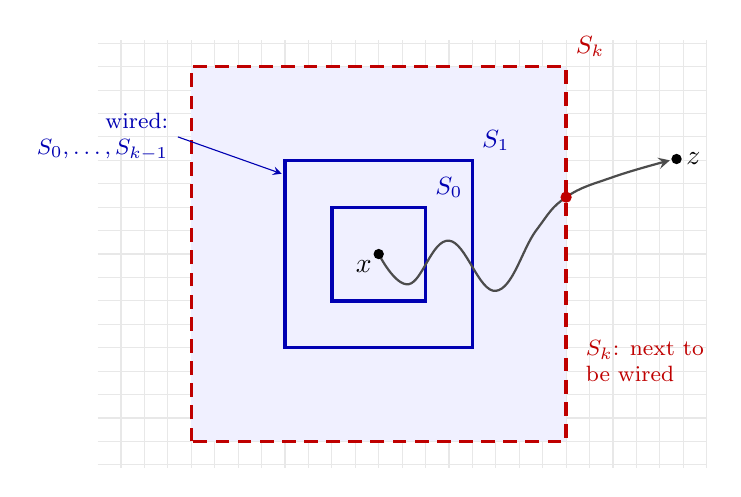
\begin{tikzpicture}[scale=0.85,
    wired/.style={very thick, blue!70!black},
    next/.style={very thick, red!75!black, dash pattern=on 5pt off 3pt},
    later/.style={thick, gray!60}]
  % lattice background
  \draw[step=0.35, gray!18] (-4.2,-3.2) grid (4.9,3.2);
  % region where all previous identifications live
  \fill[blue!6] (-2.8,-2.8) rectangle (2.8,2.8);
  % wired shells S_0, S_1 (here k = 2)
  \draw[wired] (-0.7,-0.7) rectangle (0.7,0.7);
  \draw[wired] (-1.4,-1.4) rectangle (1.4,1.4);
  % the next shell S_k
  \draw[next] (-2.8,-2.8) rectangle (2.8,2.8);
  % a path from x to z
  \draw[thick, black!70, ->, >=stealth]
    plot[smooth, tension=0.7] coordinates
      {(0,0) (0.45,-0.45) (1.05,0.2) (1.75,-0.55) (2.35,0.35) (2.8,0.85) (3.5,1.15) (4.35,1.4)};
  \fill[red!75!black] (2.8,0.85) circle (2.4pt);
  % points
  \fill (0,0) circle (2.2pt) node[below left=-1pt] {$x$};
  \fill (4.45,1.42) circle (2.2pt) node[right] {$z$};
  % labels
  \node[blue!70!black, anchor=south west, font=\small] at (0.7,0.7) {$S_0$};
  \node[blue!70!black, anchor=south west, font=\small] at (1.4,1.4) {$S_1$};
  \node[red!75!black, anchor=south west, font=\small] at (2.8,2.8) {$S_k$};
  \node[blue!70!black, align=right, font=\footnotesize, anchor=east] (w) at (-3.0,1.75)
    {wired:\\ $S_0,\dots,S_{k-1}$};
  \draw[->, >=stealth, blue!70!black] (w.east) -- (-1.45,1.2);
  \node[red!75!black, align=left, font=\footnotesize, anchor=west] at (2.95,-1.6)
    {$S_k$: next to\\ be wired};
\end{tikzpicture}
\caption{Wiring the nested shells in increasing order of radius (shown for $k=2$).
The boundaries $S_0,\dots,S_{k-1}$ (solid) are already wired, each to a single vertex;
all these identifications take place in the shaded region strictly inside $S_k$
(dashed). Every path from $x$ to $z$ still meets $S_k$ (dot), so $S_k$ separates $x$
from $z$ in the wired graph and \cref{prop:separator-wiring} applies again.}
\label{fig:nested-shells}
\end{figure}


For $1\le k\le m$ let $\mathcal P_k$ be the part of $G$ between $S_{k-1}$ and $S_k$, and let $\PP^{\rm w}_{\mathcal P_k}$
be the arboreal gas on $\mathcal P_k$ with $S_{k-1}$ and $S_k$ each wired to a single (separate) vertex.  After all
wirings, consecutive wired boundaries are articulation vertices separating the edge-disjoint pieces.  A forest on a one-vertex union is exactly a choice of a
forest on every piece: a cycle cannot use edges from two pieces, and the weights
multiply.  Consequently the forest measure factors over the pieces, and the event $x\leftrightarrow z$ requires a
crossing of every $\mathcal P_k$.  Bounding the innermost and outermost factors by $1$, and using \cref{prop:annulus}
with $\PP^{\rm w}_{\mathcal P_k}(S_{k-1}\leftrightarrow S_k)=\tau_{G_{r_{k-1}}}(a,b)$,
\begin{equation}\label{eq:annulus-product}
 \tau_G(x,z)\le\tau_{G/S_0/\cdots/S_m}(x,z)\le\prod_{k=1}^{m}\PP^{\rm w}_{\mathcal P_k}(S_{k-1}\leftrightarrow S_k)
 \le\prod_{k=0}^{m-1}C_\beta r_k^{-\kappa_\beta}.
\end{equation}
Taking logarithms,
\begin{equation}\begin{aligned}
 \log\tau_G(x,z)
 &\le m\log C_\beta
 -\kappa_\beta m\log r_0
 -\frac{\kappa_\beta\log2}{2}m(m-1).
\end{aligned}\end{equation}
Since $m=(\log D)/\log2+O_\beta(1)$, this is at most
$-a_\beta(\log D)^2+O_\beta(\log D)$.  Absorb the lower-order term into
$A_\beta$ to obtain \eqref{eq:superpoly}.

On the torus use toroidal $D$.  Every annulus used above has outer radius at most
$D/2\le L/4$, so it is contained in an embedded copy of a square lattice box and the
same proof applies.
\end{proof}

In particular,
\begin{equation}\label{eq:q-times-R}
 R^Nq_\beta(R)\longrightarrow0
 \qquad(R\to\infty)
\end{equation}
for every fixed $N$.

\section{A Simon--Lieb inequality from incident-edge correlation}\label{sec:SL}

We next extract the amount of negative dependence needed for path factorization.

\begin{lemma}[Two rooted trees]\label{lem:two-trees}
Let $A,B$ be edge-disjoint trees whose union is a forest and which share exactly one
vertex $r$.  Then
\begin{equation}\label{eq:tree-product}
 \PP_G(A\cup B\subseteq F)
 \le \PP_G(A\subseteq F)\PP_G(B\subseteq F).
\end{equation}
\end{lemma}

\begin{proof}
Root both trees at $r$.  Order the edges of $A$ so that every edge appears after all
edges on the path from $r$ to its parent endpoint.  Write this order as
$a_1,\dots,a_p$.  Then
\begin{equation}
 \PP(A\cup B\subseteq F)
 =\PP(B\subseteq F)
 \prod_{k=1}^p
 \PP(a_k\in F\mid B,A_{<k}\subseteq F).
\end{equation}
Fix $k$.  Condition on $A_{<k}$.  Contracting these edges makes the parent endpoint of
$a_k$ part of the contracted root containing $r$.  Now reveal the edges of $B$ in an
order growing outward from $r$.  Before each new edge of $B$ is revealed, the already
revealed $B$-edges have also been contracted to the same root.  Thus the next
$B$-edge and $a_k$ are incident to a common vertex in the contracted graph.
By the conditional form of incident-edge negative correlation from
\cref{prop:incident-NC}, conditioning on that next $B$-edge being present cannot
increase the inclusion probability of $a_k$.  Iterating through all edges of $B$ gives
\begin{equation}
 \PP(a_k\in F\mid B,A_{<k}\subseteq F)
 \le \PP(a_k\in F\mid A_{<k}\subseteq F).
\end{equation}
Multiplying over $k$ yields
\begin{equation}
 \PP(A\cup B\subseteq F)
 \le \PP(B\subseteq F)
 \prod_{k=1}^p\PP(a_k\in F\mid A_{<k}\subseteq F),
\end{equation}
and the product on the right is $\PP(A\subseteq F)$.
\end{proof}

If two edge-disjoint trees share two distinct vertices, their union contains a cycle,
so the acyclic-union hypothesis in the lemma is exactly what is needed in later
applications.

\begin{proposition}[Global Simon--Lieb inequality]\label{prop:Simon-Lieb}
Let $x\in D\subseteq V(G)$ and $z\notin D$.  Then
\begin{equation}\label{eq:SL}
 \tau_G(x,z)
 \le
 \sum_{\substack{u\in D,\ v\notin D\\uv\in E}}
 \PP_G(uv\in F)\,\tau_G(x,u)\,\tau_G(v,z).
\end{equation}
\end{proposition}

\begin{proof}
A forest contains at most one simple path between fixed endpoints.  Therefore the
path events are disjoint and
\begin{equation}\label{eq:path-sum}
 \tau_G(x,z)=\sum_{\gamma:x\to z\text{ simple}}\PP_G(\gamma\subseteq F).
\end{equation}
For a path $\gamma$, let $e=uv$ be its first exit edge from $D$, with $u\in D$ and
$v\notin D$.  Write
\begin{equation}
 \gamma=\gamma_-\cup\{e\}\cup\gamma_+,
\end{equation}
where $\gamma_-$ runs from $x$ to $u$ and $\gamma_+$ from $v$ to $z$.  The two edge
sets $\gamma_-$ and $\{e\}\cup\gamma_+$ are trees sharing only $u$, so
\cref{lem:two-trees} gives
\begin{equation}
 \PP(\gamma\subseteq F)
 \le \PP(\gamma_-\subseteq F)
 \PP(\{e\}\cup\gamma_+\subseteq F).
\end{equation}
Apply \cref{lem:two-trees} again to the one-edge tree $\{e\}$ and $\gamma_+$, which
share only $v$:
\begin{equation}\label{eq:path-factor}
 \PP(\gamma\subseteq F)
 \le \PP(\gamma_-\subseteq F)\PP(e\in F)
 \PP(\gamma_+\subseteq F).
\end{equation}
Fix an exit edge $e=uv$ and sum \eqref{eq:path-factor} over all full paths with that
first exit edge.  Enlarging the positive sum to all pairs consisting of a simple
$x$--$u$ path lying in $D$ and an arbitrary simple $v$--$z$ path gives an upper
bound.  The sum of the probabilities of the first family is at most $\tau_G(x,u)$,
because these path events form a subfamily of the mutually disjoint simple
$x$--$u$ path events in a forest.  The sum over all simple $v$--$z$ paths is exactly
$\tau_G(v,z)$.  Summing over exit edges proves \eqref{eq:SL}.
\end{proof}

Finally, for every edge $e$,
\begin{equation}\label{eq:single-edge-bound}
 \PP_G(e\in F)\le\frac{w_e}{1+w_e}.
\end{equation}
Indeed, condition on the status of all other edges.  If the endpoints of $e$ are
already connected, inserting $e$ would create a cycle and its conditional inclusion
probability is $0$.  Otherwise both choices are allowed and their relative weights are
$1:w_e$, so the conditional inclusion probability is $w_e/(1+w_e)$.  Averaging gives
\eqref{eq:single-edge-bound}.

\section{Finite-size criterion and exponential decay}\label{sec:exp}

Fix $\beta<\infty$ and set
\begin{equation}
 p_\beta=\frac{\beta}{1+\beta}.
\end{equation}
By \eqref{eq:q-times-R}, choose a fixed integer $R=R(\beta)$ so large that
\begin{equation}\label{eq:eta-choice}
 \eta_\beta:=(8R+4)p_\beta q_\beta(R)\le\frac12.
\end{equation}

Let $G\subseteq\ZZ^2$ be a finite nearest-neighbour subgraph with weights at most
$\beta$.  For a vertex $y$, put
\begin{equation}
 D_y=V(G)\cap B_\infty(y,R).
\end{equation}
At most $8R+4$ nearest-neighbour edges leave this square.  For every such exit edge
$uv$, with $u\in D_y$, one has $\|u-y\|_\infty=R$, so the global bound
\eqref{eq:superpoly} gives
\begin{equation}
 \tau_G(y,u)\le q_\beta(R).
\end{equation}
If $\|y-z\|_\infty>R$, apply \cref{prop:Simon-Lieb}, then
\eqref{eq:single-edge-bound} and \eqref{eq:eta-choice}, to obtain
\begin{equation}\label{eq:one-step-contraction}
 \tau_G(y,z)
 \le\eta_\beta
 \max_{\substack{v\in V(G)\\\|v-y\|_\infty\le R+1}}
 \tau_G(v,z).
\end{equation}

Let $d=\|x-z\|_\infty$ and
\begin{equation}
 n=\left\lfloor\frac{d}{R+1}\right\rfloor.
\end{equation}
Iterate \eqref{eq:one-step-contraction} $n$ times.  Before the $k$th step, the current
vertex $y_k$ satisfies
\begin{equation}
 \|y_k-z\|_\infty\ge d-k(R+1)>R
\end{equation}
for every $k<n$, so every application is legitimate.  Bound the final two-point
function by $1$.  Then
\begin{align}
 \tau_G(x,z)
 &\le\eta_\beta^n
 \le2^{-n}
 \le2\exp\left[-\frac{\log2}{R+1}\,d\right].
 \label{eq:exp-final}
\end{align}
This proves \eqref{eq:main-finite} with
\begin{equation}
 c_\beta=\frac{\log2}{R(\beta)+1}.
\end{equation}

For the torus, use toroidal distance.  If $L>2R+2$, every radius-$R$ neighbourhood
used in the one-step inequality is an ordinary lattice square, and the same proof
applies.  If $L\le2R+2$, every toroidal $\ell^\infty$ distance is at most $R+1$, so
the right side of \eqref{eq:exp-final} is at least $1$ and the estimate is automatic.
Finally $d_\infty\ge d_2/\sqrt2$ for the representative in the fundamental box, which
gives the Euclidean-distance formulation of \cref{thm:main}.

\section{Dependency map and exact references}

For convenience, we summarize which parts are external inputs and which are proved in
this note.

\begin{center}
\begin{tabular}{p{0.36\textwidth}p{0.56\textwidth}}
\hline
Ingredient & Source / proof\\
\hline
Forest vertex-field polynomial & \cite[Theorem~2.1, (2.8)]{BCHS}\\
$\HH^{0|2}$ connectivity identity & \cite[Corollary~2.2, (2.11)]{BCHS}\\
Horospherical $(t,s)$ representation & \cite[Proposition~2.9, (2.59)--(2.62)]{BCHS}\\
Moment and $s$--fermion identities & \cite[Corollary~2.10, (2.63)--(2.64)]{BCHS}\\
Pinned/unpinned relation & \cite[Proposition~2.12, (2.79)--(2.80)]{BCHS}\\
Pinned $t$-measure & \cite[Corollary~2.13, (2.84)--(2.85)]{BCHS}\\
Pinned connectivity and third moment & \cite[Corollary~2.14, (2.86)--(2.87)]{BCHS}\\
Logarithmic deformation & \cite[(4.4), Lemma~4.1, (4.5)--(4.6)]{BCHS}\\
Finite stability-preserver theorem & \cite[Theorem~1.1]{BB}\\
Rayleigh criterion for multi-affine stable polynomials & \cite[Theorem~4.1]{BBL}\\
Real stability of $P_G$ & \cref{lem:operator-identity,lem:PG-stable} of this note\\
Incident-edge negative correlation & \cref{prop:incident-NC} of this note\\
Separator-wiring monotonicity & \cref{lem:stable-separator,prop:separator-wiring} of this note\\
Effective-conductance identity & \cref{prop:conductance-identity} of this note\\
Wired-annulus bound & \cref{prop:annulus}, using \cite[Lemma~4.1]{BCHS}\\
Global Simon--Lieb inequality & \cref{lem:two-trees,prop:Simon-Lieb} of this note\\
Exponential finite-size iteration & Section~\ref{sec:exp} of this note\\
\hline
\end{tabular}
\end{center}

\appendix
\section{Prompts}

The result and this exposition was obtained with the following prompts on GPT-6 Pro:

\paragraph{Prompt 1}
Consider the arboreal gas on $\Lambda_L= (\Z/L\Z)^2$ or another approximation of $\Z^2$. Prove that for any $\beta>0$ the connection probability decays exponentially in the distance, i.e., $P[0 \leftrightarrow x] \leq C e^{-c|x|}$ when $L \gg |x|$.

You might use the representation of the arboreal as the $H^{0|2}$ nonlinear sigma model and in particular the $(t,s)$ field representation that can be found in the paper "Random spanning forests and hyperbolic symmetry" by Bauerschmidt-Crawford-Helmuth-Swan.

The corresponding statement for the $S^2$ nonlinear sigma model was proved in \url{https://github.com/openai/math/tree/main/preprints/Exponential-decay-in-two-dimensional-classical-On-models-September-23-2026}. A related statement for the $H^{2|2}$ nonlinear sigma model was proved in \url{https://arxiv.org/abs/2610.10982}.

\paragraph{Prompt 2}
Can you try to prove it assuming the conjectural negative correlation or negative association properties for the arboreal gas?

\paragraph{Prompt 3}
Now make the proof unconditional. You can either prove the negative correlation assumption or do it otherwise.

\paragraph{Lean}
The Lean version was created by Claude Opus 5.5 using Scott Armstrong's skill files.
\bigskip

Access to GPT was supported in part by a grant of access to OpenAI models through the ChatGPT for Academic Researchers program.
Access to Claude was obtained through the Claude for Scientists program.

\begin{thebibliography}{9}

\bibitem{BCHS}
R.~Bauerschmidt, N.~Crawford, T.~Helmuth, and A.~Swan,
\emph{Random Spanning Forests and Hyperbolic Symmetry},
Commun. Math. Phys. \textbf{381} (2021), 1223--1261.
DOI: \href{https://doi.org/10.1007/s00220-020-03921-y}{10.1007/s00220-020-03921-y}.
Preprint: \href{https://arxiv.org/abs/1912.04854}{arXiv:1912.04854}.

\bibitem{BB}
J.~Borcea and P.~Br\"and\'en,
\emph{The Lee--Yang and P\'olya--Schur Programs. I. Linear Operators Preserving Stability},
Invent. Math. \textbf{177} (2009), 541--569.
DOI: \href{https://doi.org/10.1007/s00222-009-0189-3}{10.1007/s00222-009-0189-3}.
Preprint: \href{https://arxiv.org/abs/0809.0401}{arXiv:0809.0401}.

\bibitem{BBL}
J.~Borcea, P.~Br\"and\'en, and T.~M.~Liggett,
\emph{Negative Dependence and the Geometry of Polynomials},
J. Amer. Math. Soc. \textbf{22} (2009), 521--567.
DOI: \href{https://doi.org/10.1090/S0894-0347-08-00618-8}{10.1090/S0894-0347-08-00618-8}.
Preprint: \href{https://arxiv.org/abs/0707.2340}{arXiv:0707.2340}.
\bibitem{Sabot} C.~Sabot, \emph{Polynomial Localization of the 2D-Vertex Reinforced Jump Process}, Electron. Commun. Probab. \textbf{26} (2021), 1--9. DOI: \href{https://doi.org/10.1214/20-ECP356}{10.1214/20-ECP356}. Preprint: \href{https://arxiv.org/abs/1907.07949}{arXiv:1907.07949}.
\end{thebibliography}

\end{document}
